\chapter{Povezivanje razvojnog sustava i računala}

Računalo i STM32 razvojni sustav dva su odvojena sustava koja moraju međusobno komunicirati i razmjenjivati podatke. Za ostvarenje njihove veze razvijena su dva programska rješenja:
\begin{enumerate}
	\item programska potpora za mikrokontroler, koja će omogućiti pokretanje i snimanje zvučnog zapisa te njegov prijenos BLE sučeljem,
	\item programska potpora za računalo, koja će ostvariti Bluetooth vezu između računala i mikrokontrolera te omogućiti prijem i pohranu primljenog audio signala.
\end{enumerate} 

\section{Programska potpora za mikrokontroler}

Dvije glavne funkcionalnosti koje mikrokontroler mora sadržavati su snimanje zvuka i njegov prijenos BLE komunikacijskim sučeljem. Za rad mikrokontrolera odabran je paket funkcija \textit{FP-AUD-BVLINKWB1} iz alata \textit{STM32Cube} koji je razvila tvrtka \textit{STMicroeletronics}. Ovaj \textit{firmware} omogućava potpuni dvosmjerni prijenos zvuka koji se prenosi BLE sučeljem koristeći Opus algoritam za kompresiju. Aplikacija sadrži upravljačke programe i posrednički softver (engl. \textit{middleware}) za BLE i digitalne MEMS mikrofone. Također uključuje kompletan Opus audio kodek kao \textit{middleware} za izvođenje dvosmjernog i simultanog prijenosa zvuka između dva STM32WB mikrokontrolera. 

\subsection{Arhitektura programske potpore za mikrokontroler}

Softver se temelji na sloju apstrakcije hardvera STM32CubeHAL za STM32 mikrokontroler. Paket funkcija opremljen je skupom \textit{middleware} komponenti za audio prijem, kompresiju i
dekompresiju, prijenos podataka preko BLE sučelja i USB-a.

Aplikacija se sastoji od sljedećih slojeva softvera:
\begin{itemize}
	\item STM32Cube HAL sloj: pruža jednostavan i modularan skup generičkih i proširenih API-ja za interakciju s gornjim slojevima aplikacije i bibliotekama. Ovi su API-ji izgrađeni na zajedničkoj arhitekturi te je moguće na njih dodavati slojeve (primjerice specifični \textit{middleware}) bez obzira na sklopovske značajke mikrokontrolera.
	\item Sloj paketa podrške za razvojni sustav (BSP): skup API-ja koji pruža programsko sučelje za periferne uređaje specifične za razvojni sustav kao što su SPI, ADC, LED i korisnički gumbi.
\end{itemize}

\begin{figure}[ht]
	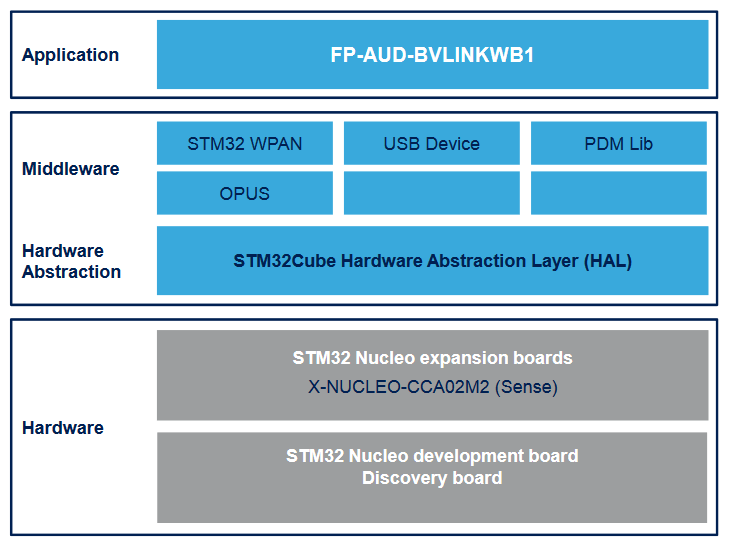
\includegraphics[width=\linewidth]{imgs/firmware_software_arch}
	\caption{Arhitektura softvera FP-AUD-BVLINKWB1}
	\label{fig:firmware_software_arch}
\end{figure}

Komponente za obradu funkcijskog paketa \textit{FP-AUD-BVLINKWB1} dizajnirane su za stvaranje bežične audio veze između modula odašiljača (Tx) i prijamnika (Rx), gdje mikrokontroler služi kao odašiljač, a računalo kao prijamnik. Cijeli lanac obrade zvuka počinje prijemom MEMS digitalnim mikrofonom i kulminira reprodukcijom zvuka na računalu.

BLE je konfiguriran za slanje paketa s maksimalnom veličinom od 150 bajtova. Ovisno o aplikaciji, kodirani bajtovi mogu biti iznad ovog praga, stoga komprimirani međuspremnik (engl. \textit{buffer}) mora biti podijeljen u više BLE paketa. Štoviše, veličina kodiranog međuspremnika može promijeniti svaki audio okvir i prijamnik mora znati njegovu duljinu da bi ga obnovio; za ovaj opseg implementiran je jednostavan protokol BLE prijenosa.

Na strani odašiljača, zvuk se dobiva digitalnim MEMS mikrofonom kao 1-bitni PDM signal i pretvara se pomoću filtra za pretvorbu PDM-u-PCM u 16-bitni PCM (pulsno-kodna modulacija). Svaki put kad je audio okvir spreman, prenosi se u algoritam kompresije: veličina kodiranog međuspremnika koju vraća Opus koder može se značajno promijeniti u skladu s parametrima Opus kodera.

\begin{figure}[ht]
	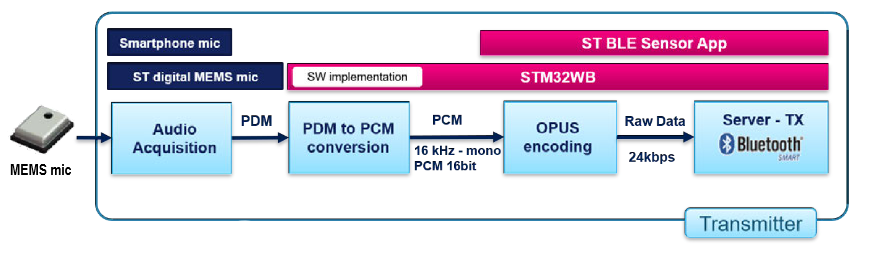
\includegraphics[width=\linewidth]{imgs/duplex_chain}
	\caption{Lanac obrade odašiljača u \textit{FP-AUD-BVLINKWB}}
	\label{fig:duplex_chain}
\end{figure}

\subsection{\textit{Middleware} za prijenos zvuka}

Budući da \textit{streaming} zvuka nije dio predefiniranog skupa profila mikrokontrolera, \textit{FP-AUD-BVLINKWB1} definira uslugu specifičnu za dobavljača pod nazivom \textit{BlueVoiceOPUS} koja je posrednik između korisničkog zvuka i  klijentskog uređaja. Ovisno o pokrenutoj aplikaciji, karakteristika se mijenja između audio ili glazbene karakteristike. Budući da \textit{streaming} glazbe nije implementiran u ovoj aplikaciji, opisane su samo audio karakteristike. 

Audio karakteristike sadrže sljedeće atribute:
\begin{itemize}
	\item \textit{Att1} - sadrži deklaraciju audio karakteristika,
	\begin{itemize}
		\item UUID: standardni 16-bitni UUID za karakterističnu deklaraciju
		\item Dozvole: R
		\item Vrijednost: svojstva za ovu karakteristiku su "\textit{notify only}", a UUID je za audio podatke
	\end{itemize}
	\item \textit{Att2} - sadrži audio podatke,
	\begin{itemize}
		\item UUID: isti UUID u zadnjih 16 bajtova vrijednosti atributa definicije karakteristike
		\item Dozvole: nema
		\item Vrijednost: stvarni audio sadržaj
	\end{itemize}
	\item \textit{Att3} - sadrži konfiguraciju karakteristika klijenta.
	\begin{itemize}
		\item UUID: standardni 16-bitni UUID za karakterističnu konfiguraciju klijenta
		\item Dozvole: R/W
		\item Vrijednost: prvi bit označava omogućenost obavijesti (0 ili 1), drugi bit omogućenost indikacija
	\end{itemize}
\end{itemize}

Usluga \textit{BlueVoiceOPUS} može implementirati odašiljač, prijamnik ili oboje u slučaju \textit{full-duplex} komunikacije. Za ovu aplikaciju potrebno je implementirati odašiljač odnosno transmiter.
Za prijenos zvuka, usluga i karakteristike moraju se kreirati pozivanjem inicijalizacijske funkcije \lstinline|BVOPUS_STM_Init()|, što uključuje funkcije \newline \lstinline|BluevoiceOPUS_AddService()| i \lstinline|BluevoiceOPUS_AddChar()|; UUID-ovi su definirani u datoteci \lstinline|bvopus_service_stm.c|.

Karakteristike se mogu dodati već postojećoj usluzi pozivanjem funkcije \newline \lstinline|BluevoiceOPUS_AddChar()| i prosljeđivanjem oznake te određene usluge kao parametra. Ako funkcija vrati \lstinline|BV_OPUS_SUCCESS|, BLE profil je ispravno kreiran.

Također, potrebno je konfigurirati Opus koder. U skladu sa traženim funkcijama, koder se može kreirati ispunjavanjem relevantne strukture: \newline \lstinline|OPUS_IF_ENC_ConfigTypeDef|.

Koder se može inicijalizirati pozivom pripadne funkcije, odnosno pozivom \newline \lstinline|BVOPUS_CodecEncInit(&EncConfigOpus)|. Ako je \textit{BlueVoiceOPUS} profil ispravno konfiguriran, funkcija će vratiti \lstinline|BV_OPUS_SUCCESS|. Ako vrati neuspjeh odnosno \lstinline|BV_OPUS_INVALID_PARAM|, neki od parametara nisu ispravni. Ovisno o odabranim parametrima, inicijalizacijska funkcija dodjeljuje količinu memorije koju relevantni API vraća interno. 

Pri inicijalizaciji podržani su sljedeći parametri:
\begin{itemize}
	\item \textit{application}: \lstinline|OPUS_APPLICATION_VOIP, OPUS_APPLICATION_AUDIO, OPUS_APPLICATION_RESTRICTED_LOWDELAY|,
	\item \textit{bitrate} [bps]: od 6000 do 510000,
	\item \textit{channels}: od 1 do 255,
	\item \textit{complexity}: od 0 do 10,
	\item \textit{ms\_frame} [ms]: 2.5, 5, 10, 20, 40, 60,
	\item \textit{sample\_freq} [Hz]: 8000, 12000, 16000, 24000, 48000.
\end{itemize}

\begin{lstlisting}[caption={Parametri za Opus koder}, language=c]
	EncConfigOpus.application = OPUS_APPLICATION_VOIP;
	/* bps */
	EncConfigOpus.bitrate = 24000; 
	/* 1 channel, mono*/
	EncConfigOpus.channels = AUDIO_CHANNELS_IN; 
	EncConfigOpus.complexity = 0;
	/* 20 ms */
	EncConfigOpus.ms_frame = AUDIO_IN_MS; 
	/* 16000 Hz */
	EncConfigOpus.sample_freq = AUDIO_IN_SAMPLING_FREQUENCY; 
\end{lstlisting}

Nakon postavljanja veze, modul koji je otkrio \textit{BlueVoiceOPUS} profil drugog modula mora omogućiti kontrolnu obavijest pozivanjem API-ja \newline \lstinline|BluevoiceOPUS_EnableCtrl_Notif(void)|. Kontrolna se obavijest zatim koristi za zahtjev za pokretanje i zaustavljanje prijenosa.

Za početak audio prijenosa, modul odašiljača mora zatražiti od prijamnika da omogući njegovu audio obavijest pozivom \lstinline|BluevoiceOPUS_SendEnableNotifReq()|. Ovaj API šalje obavijest putem kontrolne karakteristike koja sadrži dva bajta (\lstinline|{BV_OPUS_CONTROL, BV_OPUS_ENABLE_NOTIF_REQ}|). Čim čvor primi zahtjev može omogućiti audio obavijest podnositelju zahtjeva pozivom funkcije \newline \lstinline|BluevoiceOPUS_EnableAudio_Notif(void)|. Ako je obavijest ispravno omogućena, modul može započeti prijenos zvuka.

\textit{BlueVoiceOPUS} profil na ulaz prihvaća količinu PCM uzoraka jednaku veličini audio okvira postavljenoj tijekom Opus konfiguracije. Svaki put kada je audio okvir spreman, treba pozvati API \lstinline|BluevoiceOPUS_SendAudioData()| i on automatski sažima, fragmentira i šalje pakete audio podataka.

Za svaku primljenu zvučnu obavijest potrebno je pozvati funkciju \newline \lstinline|BluevoiceOPUS_ParseData()| i provjeriti vraćeni status. U slučaju uspjeha, parametar \lstinline|pcm_samples| pokazuje je li spreman kompletan audio okvir.

Prema zadanim postavkama, Opus koder je konfiguriran s promjenjivom brzinom prijenosa: svaki kodirani okvir ima  duljinu prilagođenu brzini prijenosa postavljenoj tijekom faze inicijalizacije. Maksimalna veličina BLE paketa postavljena je na 150 bajtova, a broj BLE paketa može varirati među različitim audio okvirima ili ovisno o konfiguraciji Opusa.

Protokol prijenosa \textit{BlueVoiceOPUS} modula pokazuje kada kodirani podaci počinju i završavaju tako da prijamnik može ponovno izgraditi komprimirani međuspremnik i dekodirati ga: jedan bajt se dodaje kao prvi bajt svakog BLE paketa, preostalih 19 bajtova ili više, ovisno o odabranom MTU, popunjeni su podacima kodiranim Opusom.

Sljedeće vrijednosti mogu biti bajt zaglavlja:
\begin{itemize}
	\item \lstinline|BV_OPUS_TP_START_PACKET = 0x00|
	\item \lstinline|BV_OPUS_TP_START_END_PACKET = 0x20|
	\item \lstinline|BV_OPUS_TP_MIDDLE_PACKET = 0x40|
	\item \lstinline|BV_OPUS_TP_END_PACKET = 0x80|
\end{itemize}

Protokol prijenosa u potpunosti je obrađen u \textit{BlueVoiceOPUS} usluzi.
\subsection{Opus}
Opus je otvoren i svestran audio kodek koji se može koristiti za različite vrste aplikacija kao što su \textit{streaming} govora i glazbe ili komprimirana pohrana zvuka. Skalabilnost, od uskopojasnog govora niske brzine prijenosa pri 6 kbit/s do stereo glazbe pri 510 kbit/s niske složenosti, čini ga pogodnim za širok raspon interaktivnih aplikacija.

Sastoji se od dva sloja: jedan se temelji na linearnom predviđanju (LP), a drugi se temelji na modificiranoj diskretnoj kosinusnoj transformaciji (MDCT). Opus kombinira rezultate s gubitcima i bez gubitaka. Primjerice, u govornim aplikacijama, LP tehnike poput CELP-a (engl. \textit{Code-excited linear prediction}) učinkovitije kodiraju niske frekvencije nego u tehnikama transformacijske domene kao što je MDCT.

Opus kodek se sastoji od SILK i CELT tehnologija kodiranja. Prvi koristi model temeljen na predviđanju (LPC), dok je drugi u potpunosti modeliran na MDCT transformaciji. Ova svestranost omogućuje Opusu rad u tri načina rada (SILK, CELT ili hibridni način) i osigurava višestruke konfiguracije za različite aplikacije.

\section{Programska potpora za računalo}

Glavna zadaća aplikacije na računalu je Bluetoothom primiti audio signal, prikladno ga obraditi te izravno reproducirati i pohraniti. Za računalnu programsku potporu odabrana je \textit{BlueST-SDK} biblioteka koji omogućuje jednostavan pristup podacima koje izvozi BLE uređaj s implementiranim \textit{BlueST} protokolom. \textit{BlueST} protokol lako je proširiv za podršku korisnički definiranih podataka. On također prima podatke koji dolaze iz različitih senzora kao što su inercijski senzori, senzori okoliša, informacije o bateriji, te DC i motori. Protokol implementira i serijsku konzolu preko Bluetootha koja omogućuje funkcionalnosti standardnog izlaza i standardnog ulaza te definira konfiguracijski servis za kontrolu postavki povezanih ploča. 

Korištenjem zajedničkog modela programiranja za podržane platforme, \textit{BlueST-SDK} olakšava razvoj aplikacija na Android, iOS i Linux (s instaliranim Python) sustavima i uključuje primjere aplikacija koji demonstriraju korištenje paketa za razvoj programa (\textit{Software development kit} - SDK). Paket za razvoj aplikacija na Linuxu \textit{BlueST-SDK} biblioteke koristi \textit{bluepy} Python biblioteku dostupnu na Linuxu za povezivanje s BLE uređajima.

\begin{figure}[ht]
	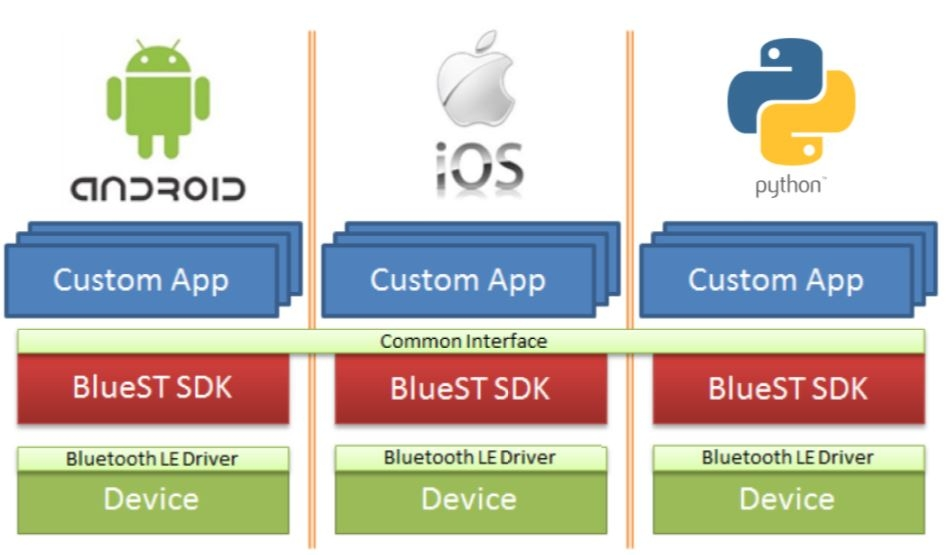
\includegraphics[width=\linewidth]{imgs/bluest_stack}
	\caption{Arhitektura aplikacije s \textit{BlueST-SDK} modulom}
	\label{fig:bluest_stack}
\end{figure}


Za razvoj aplikacije odabran je programski jezik Python na operacijskom sustavu Linux za lakše povezivanje s grafičkim korisničkim sučeljem, koje je također razvijeno u Pythonu. 

\subsection{Rad paketa za razvoj programa}

\textit{BlueST-SDK} biblioteka prikazuje samo uređaje s poljem specifičnim za dobavljača formatiranim kao što je prikazano u Tablici 3.1. Polje duljine mora biti veličine 7 ili 13 bajtova. ID uređaja je broj koji identificira tip uređaja te brojevi između 0x80 i 0xFF označavaju STM32 Nucleo razvojne sustave. Maska značajke polje bitova koje daje informaciju o značajkama koje emitira uređaj. Polje je veličine 4 bajta i svaki bit označava jednu značajku. Svaki je bit postavljen u 0 ili 1, ovisno o tome je li značajka emitirana. 

\begin{table}[ht!]
	\centering
	\caption{Oblikovanje polja specifično za dobavljača \textit{Blue-SDK} modula}
	\begin{tabular}{|c| c| c|}
		\hline
		\rowcolor{lightblue}  
		\textbf{Duljina} & \textbf{Naziv} & \textbf{Vrijednost} \\ \hline
		1 & Duljina & 0x07/0x0D \\ \hline
		1 & Tip polja & 0xFF \\ \hline
		1 & Verzija protokola & 0x01 \\ \hline
		1 & ID uređaja & 0xX \\ \hline
		4 & Maska značajke & 0xXXXXXX \\ \hline
		6 & Adresa kontrole pristupa (MAC) uređaja & 0xXXXXXXXXX \\ \hline
	\end{tabular}
\end{table}

U Tablici 3.2 nalazi se popis ključnih značajki za ovu aplikaciju i njihove maske bitova. ADPCM označava prilagodljivu diferencijalnu impulsnu kodnu modulaciju, što je varijanta diferencijalne impulsne kodne modulacije (DPCM) koja mijenja veličinu koraka kvantizacije kako bi se omogućilo daljnje smanjenje potrebne širine opsega podataka za dani omjer signal-šum. 

\begin{table}[ht!]
	\centering
	\caption{Maske bitova i pripadne karakteristike u modulu \textit{BlueST-SDK}}
	\begin{tabular}{|c| c|}
		\hline
		\rowcolor{lightblue}  
		\textbf{Duljina} & \textbf{Naziv}  \\ \hline
		26 & Razina mikrofona \\ \hline
		27 & ADPCM Audio \\ \hline
		28 & Smjer dolaska \\ \hline
		29 & \textit{Switch} \\ \hline
		30 & ADPCM sinkronizacija  \\ \hline
	\end{tabular}
\end{table}

Karakteristike kojima upravlja SDK moraju imati navedeni UUID:
\newline \texttt{XXXXXXXX-0001-11e1-ac36-0002a5d5c51}. 

SDK skenira sve usluge, tražeći karakteristike koje odgovaraju uzorku. Prvi dio UUID-a ima bitove postavljene na 1 za svaku značajku koju karakteristika izvozi. U slučaju više značajki mapiranih u jednu karakteristiku, podaci moraju biti u istom redoslijedu kao maska bitova. Podaci se trebaju formatirati kao što je prikazano u Tablici 3.3.

Prva dva bajta koriste se za slanje vremenske oznake. Ovo je osobito korisno za prepoznavanje bilo kakvog gubitka podataka. Budući da je maksimalna veličina BLE paketa 20 bajtova, maksimalna veličina polja podataka značajke je 18 bajtova.

\begin{table}[ht!]
	\centering
	\caption{Karakterističan format podataka u modulu \textit{BlueST-SDK}}
	\begin{tabular}{|c| c|}
		\hline
		\rowcolor{lightblue}  
		\textbf{Duljina} & \textbf{Naziv}  \\ \hline
		2 &  Vremenska oznaka \\ \hline
		>1 & Podatak prve značajke \\ \hline
		>1 & Podatak druge značajke \\ \hline
		... & ... \\ \hline
	\end{tabular}
\end{table}

Modul \textit{BlueST-SDK}, odnosno \textit{blue\_st\_sdk}, koristi \textit{bluepy} biblioteku za BLE povezivanje na Linuxu. Također, koristi modul \textit{concurrent.futures} za pokretanje skupova dretvi (engl. \textit{pools}) u pozadini, koje poslužuju povratne pozive promatrača. Međutim, zbog ograničenja \textit{bluepy} biblioteke, pri korištenju \textit{BlueST-SDK} modula nije moguće paralelno korištenje starih i otkrivanje novih uređaja. Isto tako, neočekivani prekid veze nije moguće odmah detektirati, nego se otkriva i obavještava putem promatrača pri izvođenju operacija čitanja i pisanja. 

\begin{figure}[ht]
	\centering
	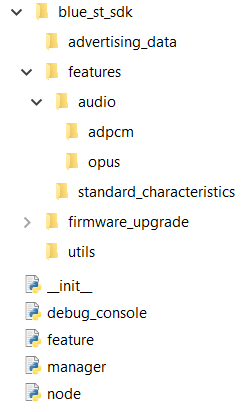
\includegraphics[scale=0.8]{imgs/sdk_folder_struct}
	\caption{Struktura modula \textit{blue\_st\_sdk}}
	\label{fig:sdk_folder_struct}
\end{figure}

Od važnijih direktorija unutar modula izdvajaju se \textit{features} i \textit{advertising\_data}. Direktorij \textit{features} sadrži klase koje implementiraju bazno sučelje \textit{Feature} iz datoteke \textit{feature.py} te svaka označava pojedinačnu značajku koju uređaj nudi, primjerice senzori za temperaturu i vlagu. Tu se također nalaze i klase koje implementiraju značajke vezane za prijenos audio signala. Direktorij \textit{advertising\_data} sadrži datoteke u kojima se nalaze klase za obradu i pohranu podataka oglasa koje šalje uređaj. 


\subsubsection{\textit{Manager} klasa}
\textit{Manager} je jedinstveni objekt koji pokreće i zaustavlja proces otkrivanja uređaja i pohranjuje dohvaćene čvorove. \textit{Manager} obavještava novootkriveni čvor putem sučelja \textit{ManagerListener}. Svaki povratni poziv (engl. \textit{callback}) izvodi se asinkrono u pozadinskoj dretvi. Pojam jedinstvenog objekta označava da postoji samo jedna, globalna instanca klase kojoj se ne može pristupiti izravno, nego isključivo putem statičke metode \lstinline|instance()|.

Također, objekt koji implementira sučelje \textit{ManagerListener} promatrač je \textit{Manager} klase, te izvršava određen skup naredbi pri svakoj promjeni \textit{Manager} objekta. Budući da bi na promjenu stanja \textit{ManagerListener} čekao u beskonačnoj petlji, odnosno ne bi obavljao nikakav koristan rad, \textit{Manager} objekt pri svakoj vlastitoj promjeni obavještava sve promatrače koji promatraju njegove promjene, odnosno poziva njihove \lstinline|update()| metode. Time se izbjegava beskonačna petlja u promatračima te izvođenje na zahtjev naredbi vezanih uz promjenu \textit{Manager} objekta.


\subsubsection{\textit{Node} klasa}
\textit{Node} klasa predstavlja udaljeni uređaj. Prihvaća značajke koje čvor odnosno uređaj emitira te omogućuje čitanje poslanih podataka, kao i njihovo slanje na uređaj. Čvor emitira sve značajke čiji je odgovarajući bit postavljen na 1 unutar poruke oglasa. Nakon što se uređaj poveže, moguće je skenirati i omogućiti dostupne karakteristike te razmjenjivati podatke vezane uz te karakteristike. Isto tako, svi promatrači zainteresirani za promjene čvora registriraju se putem \textit{NodeListener} sučelja.

Čvor može biti u jednom od sljedećih stanja:
\begin{itemize}
	\item \textit{init}: početni status,
	\item \textit{idle}: čvor čeka vezu i šalje oglasne poruke,
	\item spajanje: uspostavlja se veza sa čvorom te čvor otkriva karakteristike i usluge uređaja,
	\item spojen: veza sa čvorom je uspješno uspostavljena, 
	\item odspajanje: prekidanje veze sa čvorom koji se zatim vraća u \textit{idle} status, 
	\item izgubljen: uređaj je poslao oglašivačke podatke koji su nedohvatljivi,
	\item nedohvatljiv: veza sa čvorom je uspostavljena, no ne može se dohvatiti, 
	\item mrtav: finalni status.
\end{itemize}

\subsubsection{\textit{Feature} klasa}
\textit{Feature} klasa predstavlja podatke koje čvor emitira, odnosno jednu značajku. Svaka značajka ima niz objekata polja koji opisuju izvezene podatke. Podaci se primaju iz BLE karakteristike i pohranjuju se u objekt \textit{Sample} klase. \textit{Feature} objekti također obavještavu korisnike o promjeni podataka putem sučelja \textit{FeatureListener}.


\subsection{Povezivanje s mikrokontrolerom}

Najprije je potrebno pristupiti globalnoj instanci klase \textit{Manager} za kontrolu i skeniranje Bluetooth uređaja. Također je potrebno kreirati promatrač \textit{Manager} objekta, odnosno stvoriti instancu \textit{ManagerListener} sučelja. Korištenje bilo kojeg sučelja promatrača nije moguće bez prethodnog kreiranja klase koje nasljeđuje sučelje. 

\begin{lstlisting}[language=Python, caption={Pristup \textit{Manager} instanci i skeniranje Bluetooth uređaja}]
	manager = Manager.instance()
	manager_listener = MyManagerListener()
	manager.add_listener(manager_listener)
	manager.discover(globals.SCANNING_TIME_s)
	devices = manager.get_nodes()
\end{lstlisting}

Nakon definiranja objekata pokreće se vremenski ograničeno skeniranje dostupnih Bluetooth uređaja, koji se nakon otkrivanja pohrane u listu otkrivenih čvorova. Budući da je u ovoj aplikaciji potreban samo jedan uređaj, odabire se prvi iz liste uređaja s kojim se \textit{Manager} uređaj spaja. Nakon uspješnog spajanja i dohvata dostupnih značajki započinje snimanje zvuka. Za snimanje se mogu koristiti Opus ili AD značajke, ovisno o tome koju značajku uređaj podržava. Kao što je već ranije opisano, STM32WB5MM-DK modul podržava Opus audio kodek.

Programska podrška za snimanje zvuka je \textit{alsaaudio} modul. \textit{Advanced Linux Sound Architecture}, odnosno ALSA, pruža audio i MIDI (\textit{Musical Instrument Digital Interface}) funkcionalnost za Linux operacijski sustav. Biblioteka sadrži klase omotače (engl. \textit{wrappers}) za pristup ALSA API-ju iz Pythona. 

ALSA se sastoji od sljedećih komponenti:
\begin{itemize}
	\item skup jezgrinih upravljačkih programa koji upravljaju hardveru za zvuk iz Linux jezgre,
	\item API na razini jezgre za upravljanje ALSA uređajima, 
	\item C biblioteka za pojednostavljeni pristup hardveru za zvuk iz korisničkih aplikacija. 
\end{itemize}

Putem ALSA biblioteke definira se novi audio tok koji koristi PCM način pretvaranja binarnog zapisa u zvuk kako bi bio kompatibilan s Opus kodekom. Podaci su u 16-bitni s predznakom u \textit{little-endian} obliku, a frekvencija uzorkovanja je 16 kHz. Broj okvira koji će se upisati u pri svakoj iteraciji postavljen je na 160. 

\begin{lstlisting}[language=Python, caption={Postavljanje parametara za dekodiranje audio signala}]
	stream = alsaaudio.PCM(alsaaudio.PCM_PLAYBACK, alsaaudio.PCM_NORMAL,'default')
	stream.setformat(alsaaudio.PCM_FORMAT_S16_LE)
	stream.setchannels(globals.CHANNELS)
	stream.setrate(globals.SAMPLING_FREQ_OPUS)
	stream.setperiodsize(160)
\end{lstlisting}

Pri svakoj promjeni \textit{Feature} objekta \textit{FeatureListener} promatrač je obaviješten i \textit{Feature} poziva \textit{update()} metodu promatrača. Ta funkcija prima značajku i \textit{Sample} objekt te, ovisno o načinu obrade zvuka (ADPCM ili Opus), prikladno se obrađuje primljeni uzorak iz dobivenog \textit{Sample} objekta. Budući da je u ovoj aplikaciji korišten Opus kodek, potrebno je samo dohvatiti bajt podatka iz \textit{Sample} objekta i pohraniti ga u datoteku i/ili ga poslati na audio tok koji preusmjerava zvuk na zvučnike računala. 

\begin{figure}[ht]
	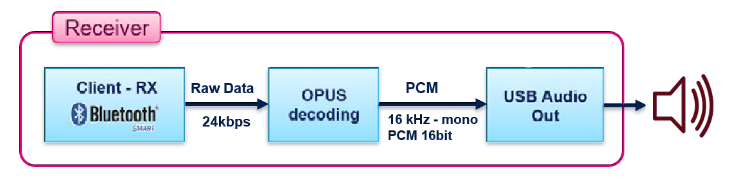
\includegraphics[width=\linewidth]{imgs/duplex_chain_2}
	\caption{Lanac obrade prijamnika u aplikaciji}
	\label{fig:duplex_chain_2}
\end{figure}

Po završetku snimanja zvuka, svi promatrači otkazuju pretplatu na subjekte koje su promatrali te se zatvore audio tokovi. \textit{Manager} objekt se odspaja od čvora i postavlja se u početno stanje.